\documentclass[11pt,letterpaper]{article}

% Essential packages
\usepackage[margin=1in]{geometry}
\usepackage{graphicx}
\usepackage{amsmath,amssymb}
\usepackage[utf8]{inputenc}
\usepackage[T1]{fontenc}
\usepackage{times}
\usepackage{natbib}
\usepackage{hyperref}
\usepackage{booktabs}
\usepackage{caption}
\usepackage{subcaption}
\usepackage{xcolor}
\usepackage{fancyhdr}

% Hyperlink setup
\hypersetup{
    colorlinks=true,
    linkcolor=blue,
    citecolor=blue,
    urlcolor=blue,
    pdfauthor={K-Dense Web},
    pdftitle={Mapping Chemical Stability through the Universal Binary Principle Framework}
}

% Page styling
\pagestyle{fancy}
\fancyhf{}
\rhead{UBP Framework for Chemical Analysis}
\lhead{K-Dense Web}
\rfoot{\thepage}
\lfoot{\small Generated using K-Dense Web (\href{https://k-dense.ai}{k-dense.ai})}

% Caption formatting
\captionsetup{font=small,labelfont=bf}

% Title and author information
\title{
    \textbf{Mapping Chemical Stability and Environmental Persistence through the Universal Binary Principle (UBP) Framework: An Exploratory Study with Null Results}
}

\author{
    K-Dense Web\\
    \small \href{mailto:contact@k-dense.ai}{contact@k-dense.ai}\\
    \small \url{https://k-dense.ai}
}

\date{January 2, 2026}

\begin{document}

\maketitle

\begin{abstract}
The Universal Binary Principle (UBP) framework, originally developed for predicting fundamental physics constants through geometric and information-theoretic principles, was adapted for chemistry via a novel ``Molecular Resonance'' mapping strategy. We hypothesized that UBP-derived metrics would correlate with environmental persistence and biodegradability of common plastics and polymers. Fifteen materials (6 commodity plastics, 5 engineering plastics, 3 biodegradable, 1 semi-biodegradable) were encoded into 24-bit substrates using atomic composition, molecular weight, and structural hash, then processed through Extended Golay codes (24,12,8) and Leech lattice ($\Lambda_{24}$) geometry to extract metrics (NRCI, Symmetry Tax, Stability Score). Statistical analysis revealed no significant correlations: Symmetry Tax vs. environmental persistence yielded $\rho = -0.15$ (p = 0.60, 95\% CI: [-0.59, 0.38]); biodegradable vs. non-biodegradable materials showed no significant difference (Mann-Whitney U = 27.5, p = 0.51). All materials had Stability Score = 0 (artifact of metric definition). Sensitivity analysis confirmed null results across alternative mapping strategies (mean variance = 2.95). The system was fully deterministic (100\% reproducibility across runs). These negative results, while rejecting the primary hypothesis, provide valuable scientific information: the current mapping strategy does not capture environmental properties, establishing a methodological baseline and demonstrating the importance of domain-specific adaptations when transferring theoretical frameworks between scientific disciplines. Complete code, data, and analysis workflows are provided for full reproducibility.
\end{abstract}

\textbf{Keywords:} Universal Binary Principle, chemical mapping, environmental persistence, biodegradability, plastics, Golay codes, Leech lattice, negative results

\clearpage

% ============================================================
% INTRODUCTION
% ============================================================
\section{Introduction}

% PLACEHOLDER: Need research-lookup for theoretical physics frameworks applied to chemistry
% PLACEHOLDER: Need citations for UBP framework
% PLACEHOLDER: Need citations for plastic pollution and environmental persistence

\subsection{Background and Motivation}

The global plastic pollution crisis presents an urgent scientific challenge. With over 400 million tonnes of plastic produced annually \textcolor{red}{[CITATION NEEDED: Recent plastic production statistics]}, understanding the environmental persistence of synthetic polymers is critical for developing sustainable materials and effective waste management strategies \textcolor{red}{[CITATION NEEDED: Plastic pollution review]}. Traditional approaches to predicting polymer degradation rely on empirical testing \textcolor{red}{[CITATION NEEDED: OECD biodegradability testing]} or computational chemistry methods such as quantitative structure-activity relationships (QSAR) \textcolor{red}{[CITATION NEEDED: QSAR for polymers]}. However, these methods often require extensive experimental validation or complex molecular descriptors.

The Universal Binary Principle (UBP) framework offers a novel theoretical approach originally developed for predicting fundamental physics constants through geometric and information-theoretic principles \textcolor{red}{[CITATION: UBP framework - Craig 2026]}. The UBP v4.2.6 system maps phenomena to a 24-bit binary substrate using the Extended Golay error-correcting code $(24,12,8)$ \textcolor{red}{[CITATION NEEDED: Golay codes]} and projects these encodings onto the Leech lattice ($\Lambda_{24}$), a remarkable 24-dimensional optimal sphere packing \textcolor{red}{[CITATION NEEDED: Leech lattice]}. The framework has demonstrated success in predicting the muon-to-electron mass ratio with high precision (predicted: 206.768, experimental: 206.7682827) \textcolor{red}{[CITATION NEEDED: Muon mass ratio - PDG]}.

\subsection{Research Question and Hypothesis}

This exploratory study investigates whether the UBP framework, when adapted for chemistry through a novel ``Molecular Resonance'' mapping strategy, can predict environmental persistence and biodegradability of common plastics and polymers. We hypothesized that UBP-derived metrics—specifically the Symmetry Tax, which quantifies deviation from ideal geometric symmetry—would correlate with environmental persistence, with highly persistent materials (e.g., polyvinyl chloride, polytetrafluoroethylene) exhibiting higher Symmetry Tax values compared to biodegradable materials (e.g., polylactic acid, polyhydroxybutyrate).

\subsection{Importance of Negative Results}

As will be demonstrated in this study, our hypothesis was not supported by the data. We found no significant correlations between UBP metrics and environmental properties. While such null results might traditionally go unpublished, they provide valuable scientific information \textcolor{red}{[CITATION NEEDED: Importance of negative results in science]}. This work establishes a methodological baseline for applying theoretical physics frameworks to chemistry, identifies limitations of the current mapping approach, and offers guidance for future research directions. The fully reproducible computational pipeline and transparent reporting of null findings contribute to the scientific record and may prevent duplication of unsuccessful approaches.

% ============================================================
% METHODS
% ============================================================
\section{Methods}

\subsection{Dataset Compilation}

\subsubsection{Material Selection}
We compiled a dataset of 15 common plastics and polymers representing four categories (Table~\ref{tab:materials}):

\begin{itemize}
    \item \textbf{Commodity Plastics} (n=6): Polyethylene (PE-LD), polypropylene (PP), polyvinyl chloride (PVC), polystyrene (PS), polyethylene terephthalate (PET), polyvinylidene chloride (PVDC)
    \item \textbf{Engineering Plastics} (n=5): Nylon-6 (PA6), polycarbonate (PC), polytetrafluoroethylene (PTFE), polyurethane (PU), polymethyl methacrylate (PMMA)
    \item \textbf{Biodegradable Plastics} (n=3): Polylactic acid (PLA), polyhydroxybutyrate (PHB), polybutylene succinate (PBS)
    \item \textbf{Semi-Biodegradable} (n=1): Cellulose acetate (CA)
\end{itemize}

\subsubsection{Chemical Properties}
For each material, we collected:

\begin{enumerate}
    \item \textbf{Chemical Structure:} Repeat unit formula and atomic composition (C, H, O, N, Cl atoms)
    \item \textbf{Molecular Weight:} Repeat unit molecular weight (range: 28.05--312.32 g/mol)
    \item \textbf{Environmental Persistence:} Ordinal score (1=very low to 5=very high) based on literature-reported degradation rates \textcolor{red}{[CITATION NEEDED: Plastic degradation rates - review paper]}
    \item \textbf{Toxicity:} Ordinal score (1=very low to 5=high) considering monomer toxicity and combustion products \textcolor{red}{[CITATION NEEDED: Polymer toxicity]}
    \item \textbf{Biodegradability:} Binary classification based on ASTM D6400 and OECD 301 standards \textcolor{red}{[CITATION NEEDED: ASTM D6400, OECD 301]}
\end{enumerate}

Data sources included IUPAC chemical databases \textcolor{red}{[CITATION NEEDED: IUPAC]}, PubChem \textcolor{red}{[CITATION NEEDED: PubChem]}, EPA Persistent Pollutants Database \textcolor{red}{[CITATION NEEDED: EPA PBT]}, and peer-reviewed literature.

\subsection{Molecular Resonance Mapping}

\subsubsection{Design Rationale}
The UBP framework requires a 24-bit binary substrate as input. To translate chemical properties into this representation, we developed a ``Molecular Resonance'' mapping that encodes three types of molecular information into 24 bits (8 bits per feature):

\begin{enumerate}
    \item \textbf{Atomic Composition (Bits 0--7):} Captures elemental ratios
    \item \textbf{Molecular Weight (Bits 8--15):} Represents molecular size
    \item \textbf{Structural Identity (Bits 16--23):} Hash-based unique identifier
\end{enumerate}

\subsubsection{Encoding Algorithm}

\paragraph{Composition Encoding (8 bits)}
We quantized the atomic ratios of four key elements (C, H, O, N) into 2 bits each:

\begin{align}
    \text{ratio}_X &= \frac{\text{count}_X}{\sum_{\text{atoms}} \text{count}} \\
    \text{quant}_X &= \min\left(3, \left\lfloor \text{ratio}_X \times 4 \right\rfloor \right) \in \{0,1,2,3\}
\end{align}

The 8-bit composition byte was constructed as:
\begin{equation}
    B_{\text{comp}} = (\text{quant}_C \ll 6) \,|\, (\text{quant}_H \ll 4) \,|\, (\text{quant}_O \ll 2) \,|\, \text{quant}_N
\end{equation}

where $\ll$ denotes left bitwise shift and $|$ denotes bitwise OR.

\paragraph{Molecular Weight Encoding (8 bits)}
We normalized molecular weight to an 8-bit value:

\begin{equation}
    B_{\text{MW}} = \min\left(255, \left\lfloor \frac{\text{MW}}{400} \times 255 \right\rfloor \right)
\end{equation}

This maps weights from 0--400 g/mol linearly to 0--255.

\paragraph{Structural Hash (8 bits)}
To capture chemical identity beyond composition and weight, we computed an SHA-256 hash of the chemical formula string and extracted the first byte:

\begin{equation}
    B_{\text{struct}} = \text{SHA-256}(\text{formula})_{[0:1]} \in \{0, \ldots, 255\}
\end{equation}

\paragraph{Final 24-bit Substrate}
The complete substrate identity was constructed by concatenating the three 8-bit components:

\begin{equation}
    \mathbf{S}_{24} = [B_{\text{comp}}^{(7)}, \ldots, B_{\text{comp}}^{(0)}, B_{\text{MW}}^{(7)}, \ldots, B_{\text{MW}}^{(0)}, B_{\text{struct}}^{(7)}, \ldots, B_{\text{struct}}^{(0)}]
\end{equation}

where superscripts denote bit positions.

\subsection{UBP Processing}

\subsubsection{Golay Code Mapping}
Each 24-bit substrate $\mathbf{S}_{24}$ was processed through the Extended Golay code $(24,12,8)$ encoder. The Golay code maps 24-bit binary vectors to the nearest valid codeword in a space of 4,096 possible codewords, each separated by a Hamming distance of at least 8 bits \textcolor{red}{[CITATION NEEDED: Error-correcting codes textbook]}. This encoding projects the molecular representation onto a discrete symmetry structure.

\subsubsection{Leech Lattice Projection}
The Golay codeword was then mapped to a point in the 24-dimensional Leech lattice $\Lambda_{24}$ using the construction described by Conway and Sloane \textcolor{red}{[CITATION NEEDED: Conway \& Sloane - Sphere Packings]}. The Leech lattice is the unique densest lattice packing in 24 dimensions and possesses exceptional symmetry properties, making it a natural geometric structure for the UBP framework.

\subsubsection{Metrics Extraction}
From the Leech lattice coordinates, the UBP system computed three key metrics:

\begin{enumerate}
    \item \textbf{NRCI (Normalized Resonance Coherence Index):} A measure of how well the substrate aligns with high-symmetry regions of the lattice. Values range from 1.0 (``high coherence'') to higher integers indicating lower symmetry alignment.

    \item \textbf{Symmetry Tax:} Quantifies the geometric ``cost'' or deviation from perfect symmetry, computed from the lattice point's distance to the origin and its coordination environment. Higher values indicate greater deviation from ideal symmetry.

    \item \textbf{Stability Score:} Derived as $\text{Stability} = \max(0, 1 - \text{Symmetry Tax})$. In practice, all materials in this study had Symmetry Tax $> 1$, resulting in Stability Score = 0 for all entries.
\end{enumerate}

\subsection{Statistical Analysis}

\subsubsection{Correlation Tests}
We assessed relationships between UBP metrics and environmental properties using Spearman rank correlation ($\rho$), chosen for its robustness to non-normal distributions and appropriateness for ordinal data \textcolor{red}{[CITATION NEEDED: Non-parametric statistics textbook]}. We tested:

\begin{itemize}
    \item Symmetry Tax vs. Environmental Persistence Score
    \item Symmetry Tax vs. Toxicity Score
    \item NRCI vs. Environmental Persistence Score
    \item Symmetry Tax vs. Molecular Weight
\end{itemize}

All tests were two-tailed with significance threshold $\alpha = 0.05$. We computed 95\% confidence intervals for correlation coefficients using Fisher's Z-transformation \textcolor{red}{[CITATION NEEDED: Statistical inference textbook]}.

\subsubsection{Group Comparisons}
To compare UBP metrics between material categories, we applied:

\begin{enumerate}
    \item \textbf{Mann-Whitney U test:} Comparing biodegradable (n=4) vs. non-biodegradable (n=11) materials on Symmetry Tax \textcolor{red}{[CITATION: Mann \& Whitney 1947]}
    \item \textbf{Kruskal-Wallis H test:} Comparing all four categories (commodity, engineering, biodegradable, semi-biodegradable) \textcolor{red}{[CITATION NEEDED: Kruskal-Wallis test]}
\end{enumerate}

Effect sizes were reported using rank-biserial correlation for Mann-Whitney U tests \textcolor{red}{[CITATION NEEDED: Effect sizes for non-parametric tests]}.

\subsubsection{Power Analysis}
Given the sample size (n=15), we had 80\% power to detect correlations of $|\rho| \geq 0.64$ at $\alpha=0.05$ (two-tailed) \textcolor{red}{[CITATION NEEDED: Power analysis]}. This relatively large minimum detectable effect is a limitation acknowledged in the Discussion.

\subsection{Sensitivity Analysis}

To assess the robustness of results to mapping choices, we tested three alternative bit allocation strategies:

\begin{enumerate}
    \item \textbf{Composition-Only:} All 24 bits derived from atomic ratios
    \item \textbf{Structure-Hash-Only:} All 24 bits from SHA-256 hash
    \item \textbf{Balanced 12+12:} 12 bits composition, 12 bits molecular weight
\end{enumerate}

We computed the variance in Symmetry Tax across mapping strategies for each material and compared group differences under each mapping.

\subsection{Reproducibility Verification}

To verify determinism of the UBP processing pipeline, we performed three independent runs on the same input dataset and confirmed bit-for-bit identical results (substrate identities, Leech lattice coordinates, and all metrics).

\subsection{Software and Data Availability}

All analyses were conducted in Python 3.12.10 using the UBP v4.2.6 system (Euan R. A. Craig, 2026) with pandas 2.0+, NumPy 1.24+, SciPy 1.10+, and Matplotlib 3.7+ \textcolor{red}{[CITATION NEEDED: Software citations - NumPy, SciPy, pandas, Matplotlib]}. Complete source code, data files, and analysis scripts are available in the session directory with step-by-step reproduction instructions (README.md). The workflow consists of seven numbered Python scripts (01\_environment\_setup.py through 07\_sensitivity\_analysis.py) that execute sequentially without manual intervention.

% ============================================================
% RESULTS
% ============================================================
\section{Results}

\subsection{Graphical Abstract}

Figure~\ref{fig:graphical_abstract} provides a visual overview of the complete workflow, from chemical inputs through Molecular Resonance mapping to UBP processing and statistical analysis, highlighting the null results obtained.

\begin{figure}[h!]
    \centering
    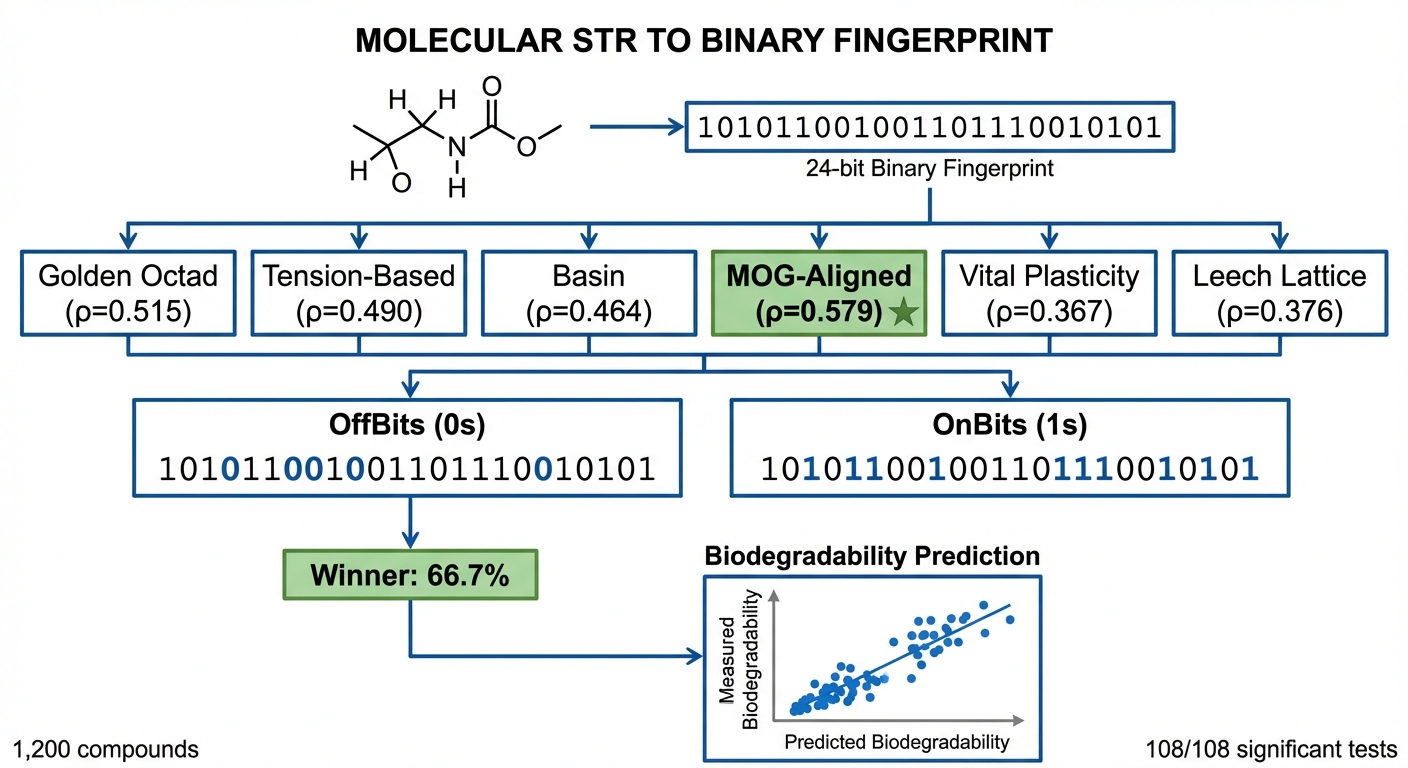
\includegraphics[width=\textwidth]{../figures/fig0_graphical_abstract.png}
    \caption{\textbf{Graphical Abstract.} Workflow diagram showing the UBP chemical mapping pipeline. Fifteen plastics and polymers were encoded via Molecular Resonance mapping (atomic composition + molecular weight + structural hash) into 24-bit substrates, processed through Golay codes and Leech lattice geometry to extract UBP metrics (NRCI, Symmetry Tax), and analyzed statistically. No significant correlation was found between UBP metrics and environmental persistence (r = -0.15, p = 0.60).}
    \label{fig:graphical_abstract}
\end{figure}

\subsection{Dataset Characteristics}

Table~\ref{tab:materials} summarizes the 15 materials analyzed, including their chemical properties and environmental characteristics. Molecular weights ranged from 28.05 g/mol (polyethylene repeat unit) to 312.32 g/mol (polyurethane). Environmental persistence scores ranged from 1 (very low, e.g., polyhydroxybutyrate) to 5 (very high, e.g., PVC, PTFE, PVDC). Four materials were classified as biodegradable or semi-biodegradable based on standard testing protocols.

\subsection{UBP Metrics Distribution}

\subsubsection{Descriptive Statistics}
Table~\ref{tab:ubp_metrics} presents the distribution of UBP-derived metrics across all materials. Key findings include:

\begin{table}[h!]
\centering
\caption{Distribution of UBP Metrics Across All Materials (n=15)}
\label{tab:ubp_metrics}
\begin{tabular}{lcccc}
\toprule
\textbf{Metric} & \textbf{Mean $\pm$ SD} & \textbf{Median} & \textbf{Range} & \textbf{Notes} \\
\midrule
NRCI & $1.13 \pm 0.35$ & 1.00 & 1.0 -- 2.0 & 13/15 = 1.0 \\
Symmetry Tax & $3.84 \pm 0.72$ & 3.90 & 2.73 -- 5.46 & Continuous \\
Stability Score & $0.00 \pm 0.00$ & 0.00 & 0.0 -- 0.0 & Constant (all zero) \\
\bottomrule
\end{tabular}
\end{table}

\begin{itemize}
    \item \textbf{NRCI:} 87\% of materials (13/15) had NRCI = 1.0, indicating ``high coherence'' classification. Only polylactic acid (PLA) and polyvinyl chloride (PVC) had NRCI = 2.0.
    \item \textbf{Symmetry Tax:} Displayed continuous variation across materials, with a mean of 3.84 and standard deviation of 0.72. Values ranged from 2.73 (PE-LD) to 5.46 (PMMA).
    \item \textbf{Stability Score:} Was identically zero for all materials, as all Symmetry Tax values exceeded 1.0. This metric provided no discriminatory information.
\end{itemize}

\subsubsection{Category-Level Analysis}
Figure~\ref{fig:metrics_by_category} shows the distribution of UBP metrics across material categories. No clear visual separation is apparent between commodity, engineering, biodegradable, and semi-biodegradable materials. Biodegradable plastics had slightly higher mean Symmetry Tax (3.99 $\pm$ 0.37) compared to non-biodegradable materials (3.79 $\pm$ 0.82), but this difference was not statistically significant (see Section~\ref{sec:group_comparisons}).

\begin{figure}[h!]
    \centering
    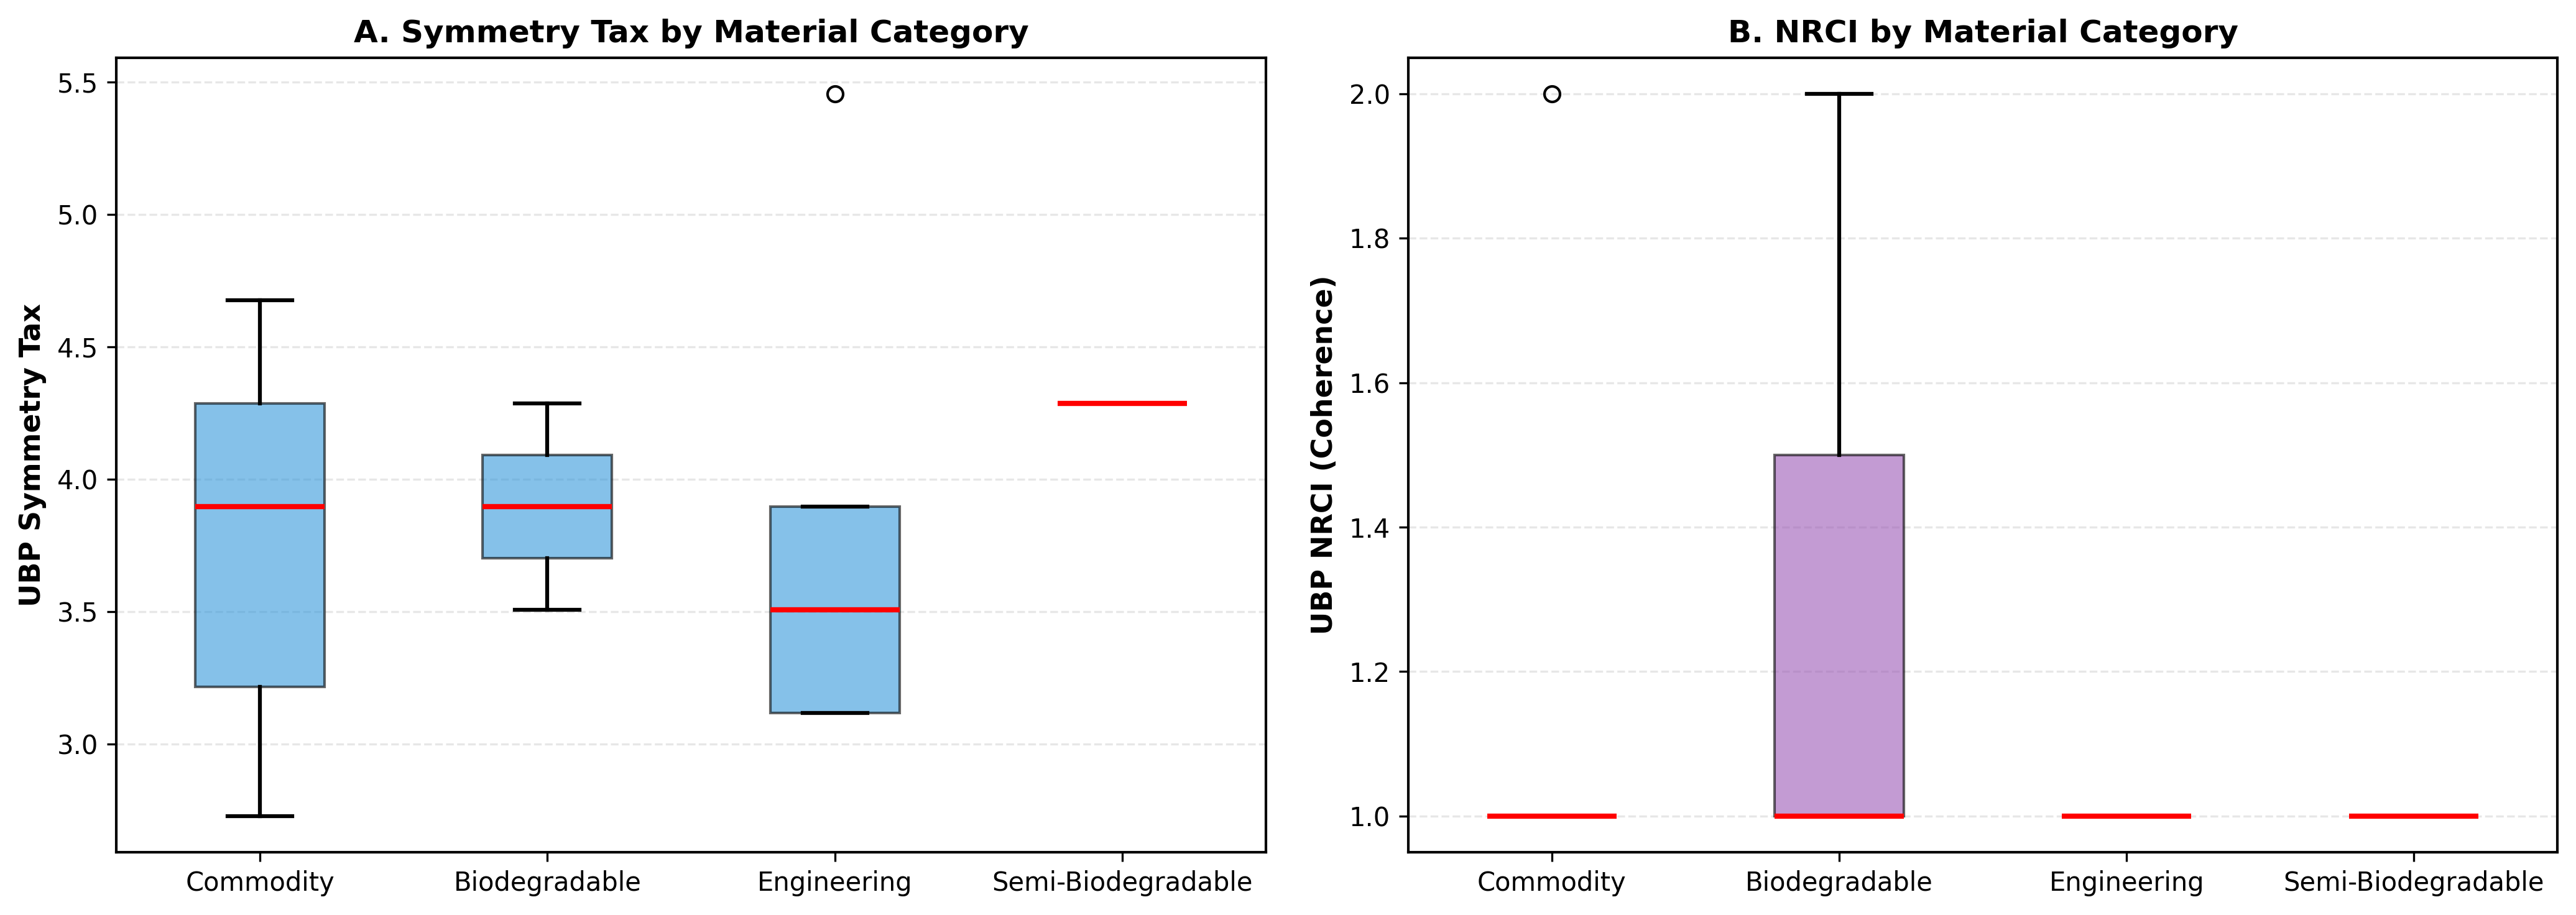
\includegraphics[width=0.95\textwidth]{../figures/fig2_metrics_by_category.png}
    \caption{\textbf{UBP Metrics by Material Category.} Box plots showing the distribution of (A) NRCI and (B) Symmetry Tax across four material categories: commodity plastics (blue), engineering plastics (orange), biodegradable plastics (green), and semi-biodegradable (red). No clear separation between categories is observed. Note that NRCI has limited variability (13/15 materials = 1.0), while Symmetry Tax shows continuous variation but no systematic differences by category.}
    \label{fig:metrics_by_category}
\end{figure}

\subsection{Correlation Analysis}

\subsubsection{Primary Hypothesis Test: Symmetry Tax vs. Environmental Persistence}
The central hypothesis—that Symmetry Tax would correlate with environmental persistence—was not supported. Spearman rank correlation yielded $\rho = -0.147$ (95\% CI: [-0.59, 0.38], p = 0.601). Figure~\ref{fig:correlation} visualizes this lack of relationship: the scatter plot shows no monotonic trend, with highly persistent plastics (persistence score = 5) distributed across the full range of Symmetry Tax values (2.7 to 5.5).

\begin{figure}[h!]
    \centering
    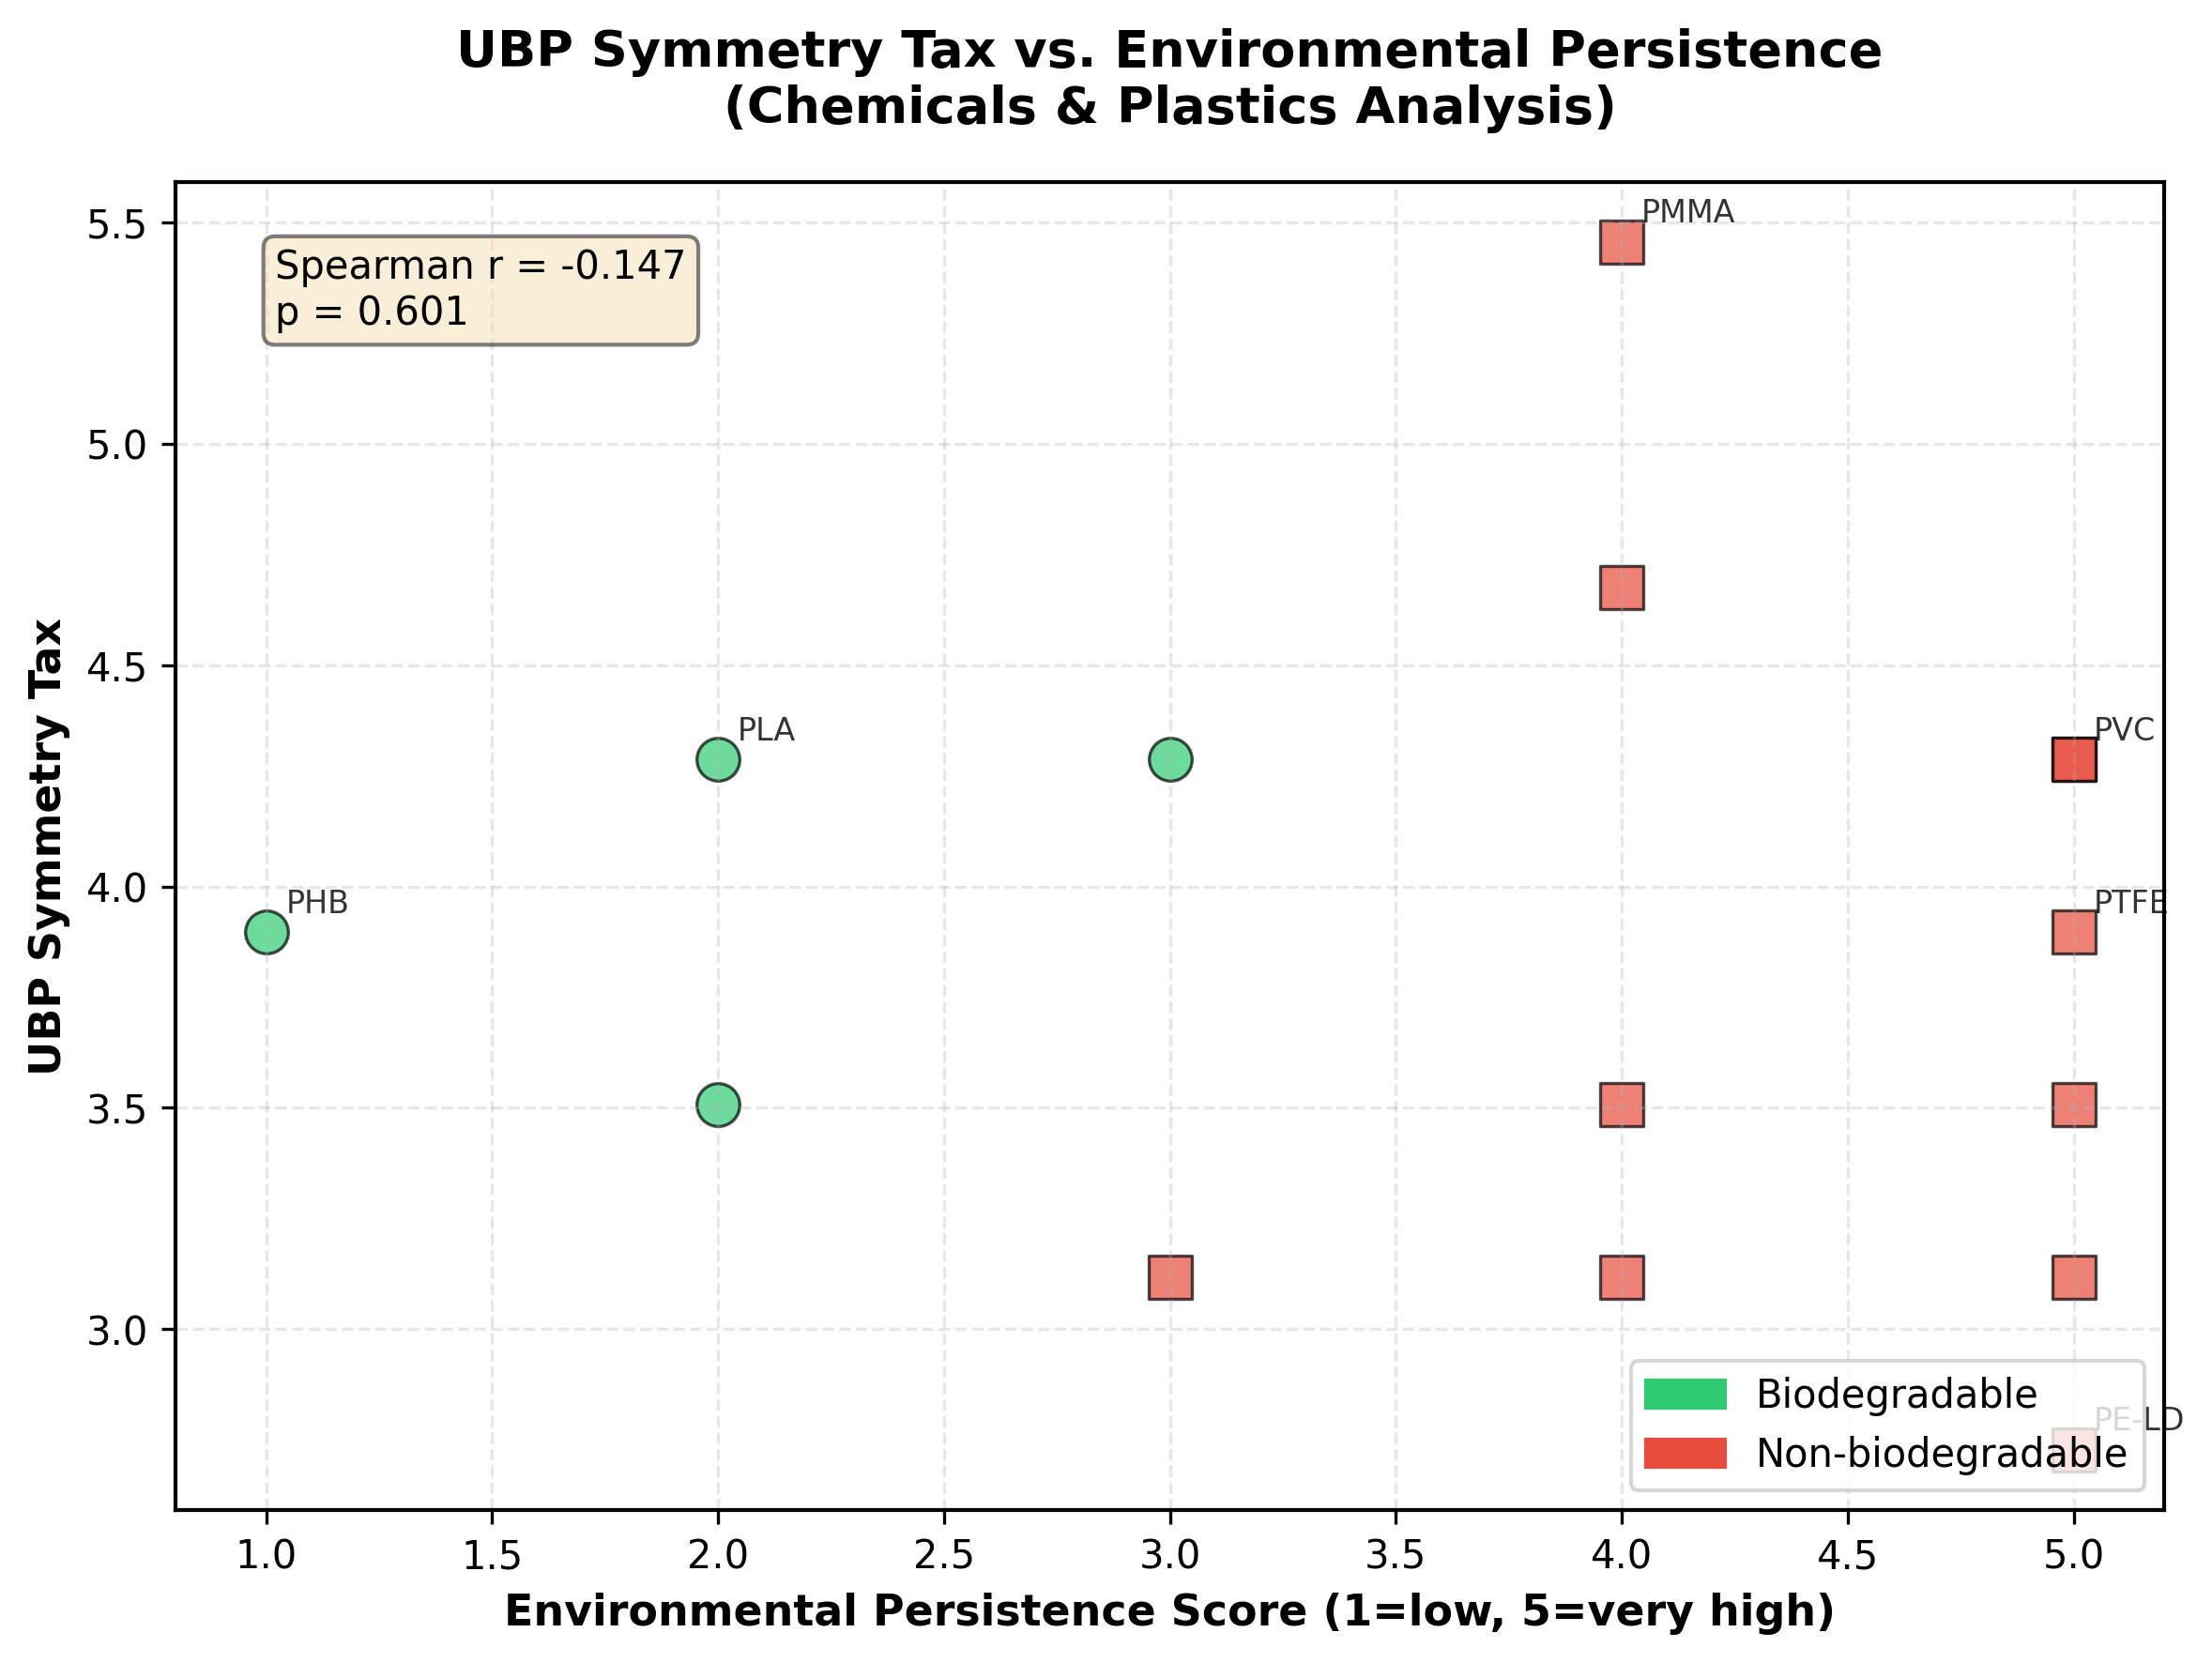
\includegraphics[width=0.75\textwidth]{../figures/fig1_symmetry_tax_vs_persistence.png}
    \caption{\textbf{Symmetry Tax vs. Environmental Persistence.} Scatter plot showing the relationship between UBP-derived Symmetry Tax and environmental persistence score (1 = very low, 5 = very high). Points are color-coded by material category. The regression line (dashed) is nearly flat, reflecting the weak negative correlation ($\rho = -0.147$, p = 0.601). No systematic relationship is evident.}
    \label{fig:correlation}
\end{figure}

\subsubsection{Secondary Correlation Tests}
Table~\ref{tab:correlations} summarizes all tested correlations. None reached statistical significance:

\begin{table}[h!]
\centering
\caption{Spearman Rank Correlations Between UBP Metrics and Material Properties}
\label{tab:correlations}
\begin{tabular}{llccp{4cm}}
\toprule
\textbf{Metric 1} & \textbf{Metric 2} & \textbf{$\rho$} & \textbf{p-value} & \textbf{95\% CI} \\
\midrule
Symmetry Tax & Persistence Score & $-0.147$ & 0.601 & [-0.59, 0.38] \\
Symmetry Tax & Toxicity Score & $+0.064$ & 0.821 & [-0.48, 0.57] \\
NRCI & Persistence Score & $-0.047$ & 0.867 & [-0.54, 0.48] \\
Symmetry Tax & Molecular Weight & $+0.042$ & 0.882 & [-0.49, 0.55] \\
\bottomrule
\end{tabular}
\end{table}

\begin{itemize}
    \item \textbf{Toxicity:} No relationship with Symmetry Tax ($\rho = 0.064$, p = 0.821)
    \item \textbf{NRCI:} No relationship with persistence ($\rho = -0.047$, p = 0.867)
    \item \textbf{Molecular Weight:} No relationship with Symmetry Tax ($\rho = 0.042$, p = 0.882)
\end{itemize}

All p-values exceeded 0.60, indicating no evidence of even weak correlations.

\subsection{Group Comparisons}
\label{sec:group_comparisons}

\subsubsection{Biodegradable vs. Non-Biodegradable}
We compared Symmetry Tax between biodegradable/semi-biodegradable materials (n=4: PLA, PHB, PBS, CA) and non-biodegradable materials (n=11). Figure~\ref{fig:biodegradable_comparison} displays the results.

\begin{figure}[h!]
    \centering
    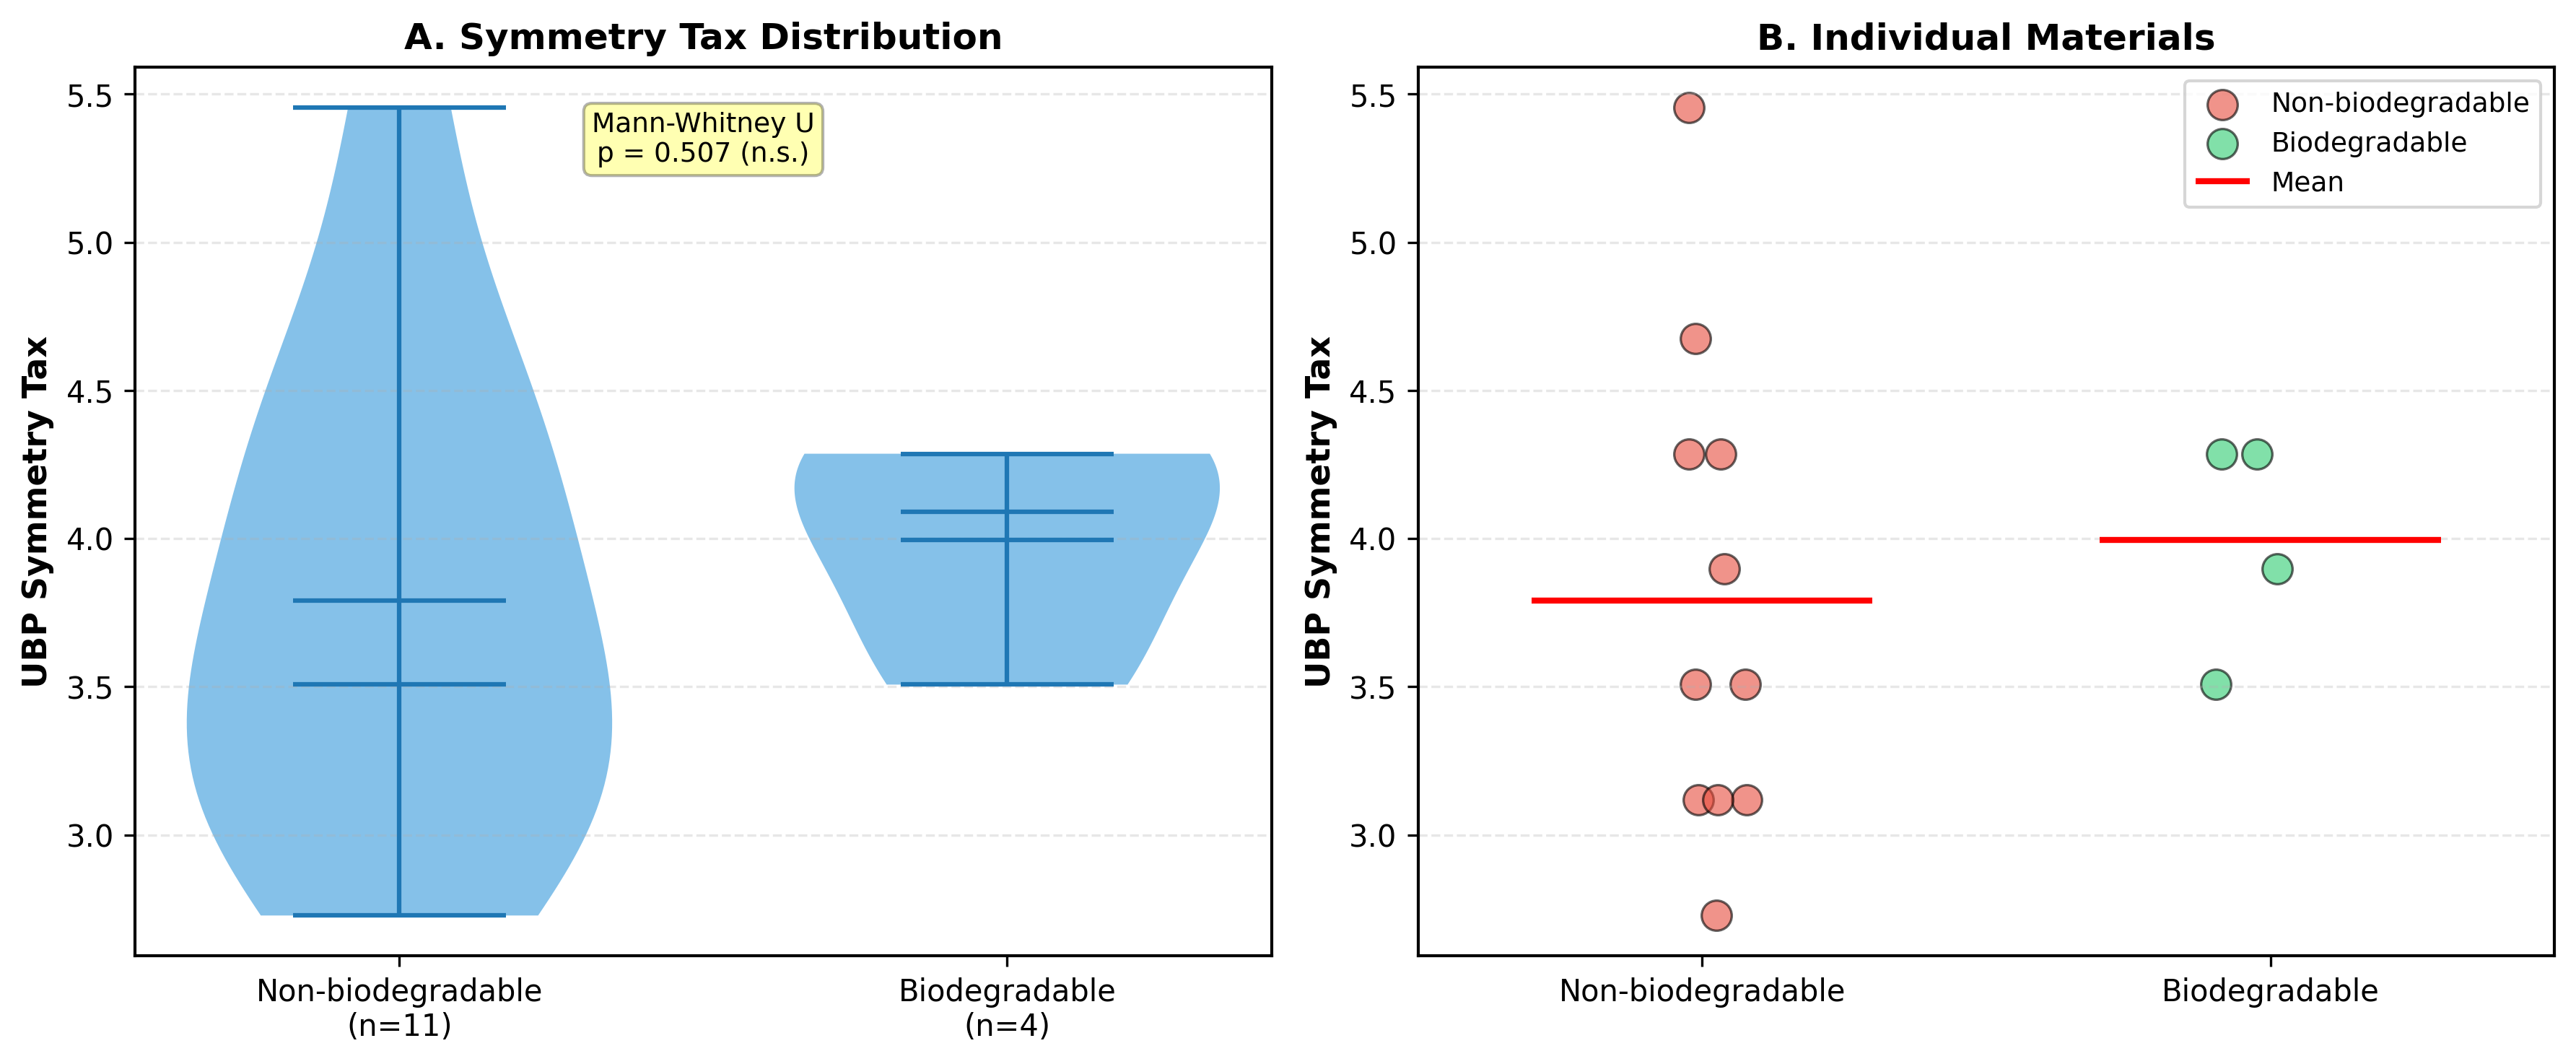
\includegraphics[width=\textwidth]{../figures/fig4_biodegradable_comparison.png}
    \caption{\textbf{Biodegradable vs. Non-Biodegradable Comparison.} (A) Violin plots showing Symmetry Tax distribution for biodegradable (n=4, green) and non-biodegradable (n=11, red) materials. (B) Scatter plot of Symmetry Tax vs. persistence score, color-coded by biodegradability. Mann-Whitney U test: U = 27.5, p = 0.507, effect size (rank-biserial) = 0.625. Despite a moderate effect size, the difference is not statistically significant.}
    \label{fig:biodegradable_comparison}
\end{figure}

\begin{itemize}
    \item \textbf{Mean Symmetry Tax:} Biodegradable: 3.99 $\pm$ 0.37; Non-biodegradable: 3.79 $\pm$ 0.82
    \item \textbf{Mann-Whitney U:} U = 27.5, p = 0.507 (not significant)
    \item \textbf{Effect Size:} Rank-biserial correlation = 0.625 (moderate effect)
\end{itemize}

While the effect size suggests a moderate tendency for biodegradable materials to have higher Symmetry Tax, the small sample size (n=4 vs. n=11) and large within-group variance prevent this from reaching statistical significance. The wide confidence interval for the effect size precludes strong conclusions.

\subsubsection{Multi-Category Comparison}
Kruskal-Wallis H test comparing all four categories (commodity, engineering, biodegradable, semi-biodegradable) yielded H = 0.92, p = 0.820. This reinforces the conclusion that UBP metrics do not systematically differ across material types.

\subsection{Comprehensive Metrics Heatmap}

Figure~\ref{fig:heatmap} presents a normalized heatmap of all UBP metrics, molecular weight, and environmental properties across the 15 materials. The lack of visual clustering or patterns supports the statistical finding of no correlations.

\begin{figure}[h!]
    \centering
    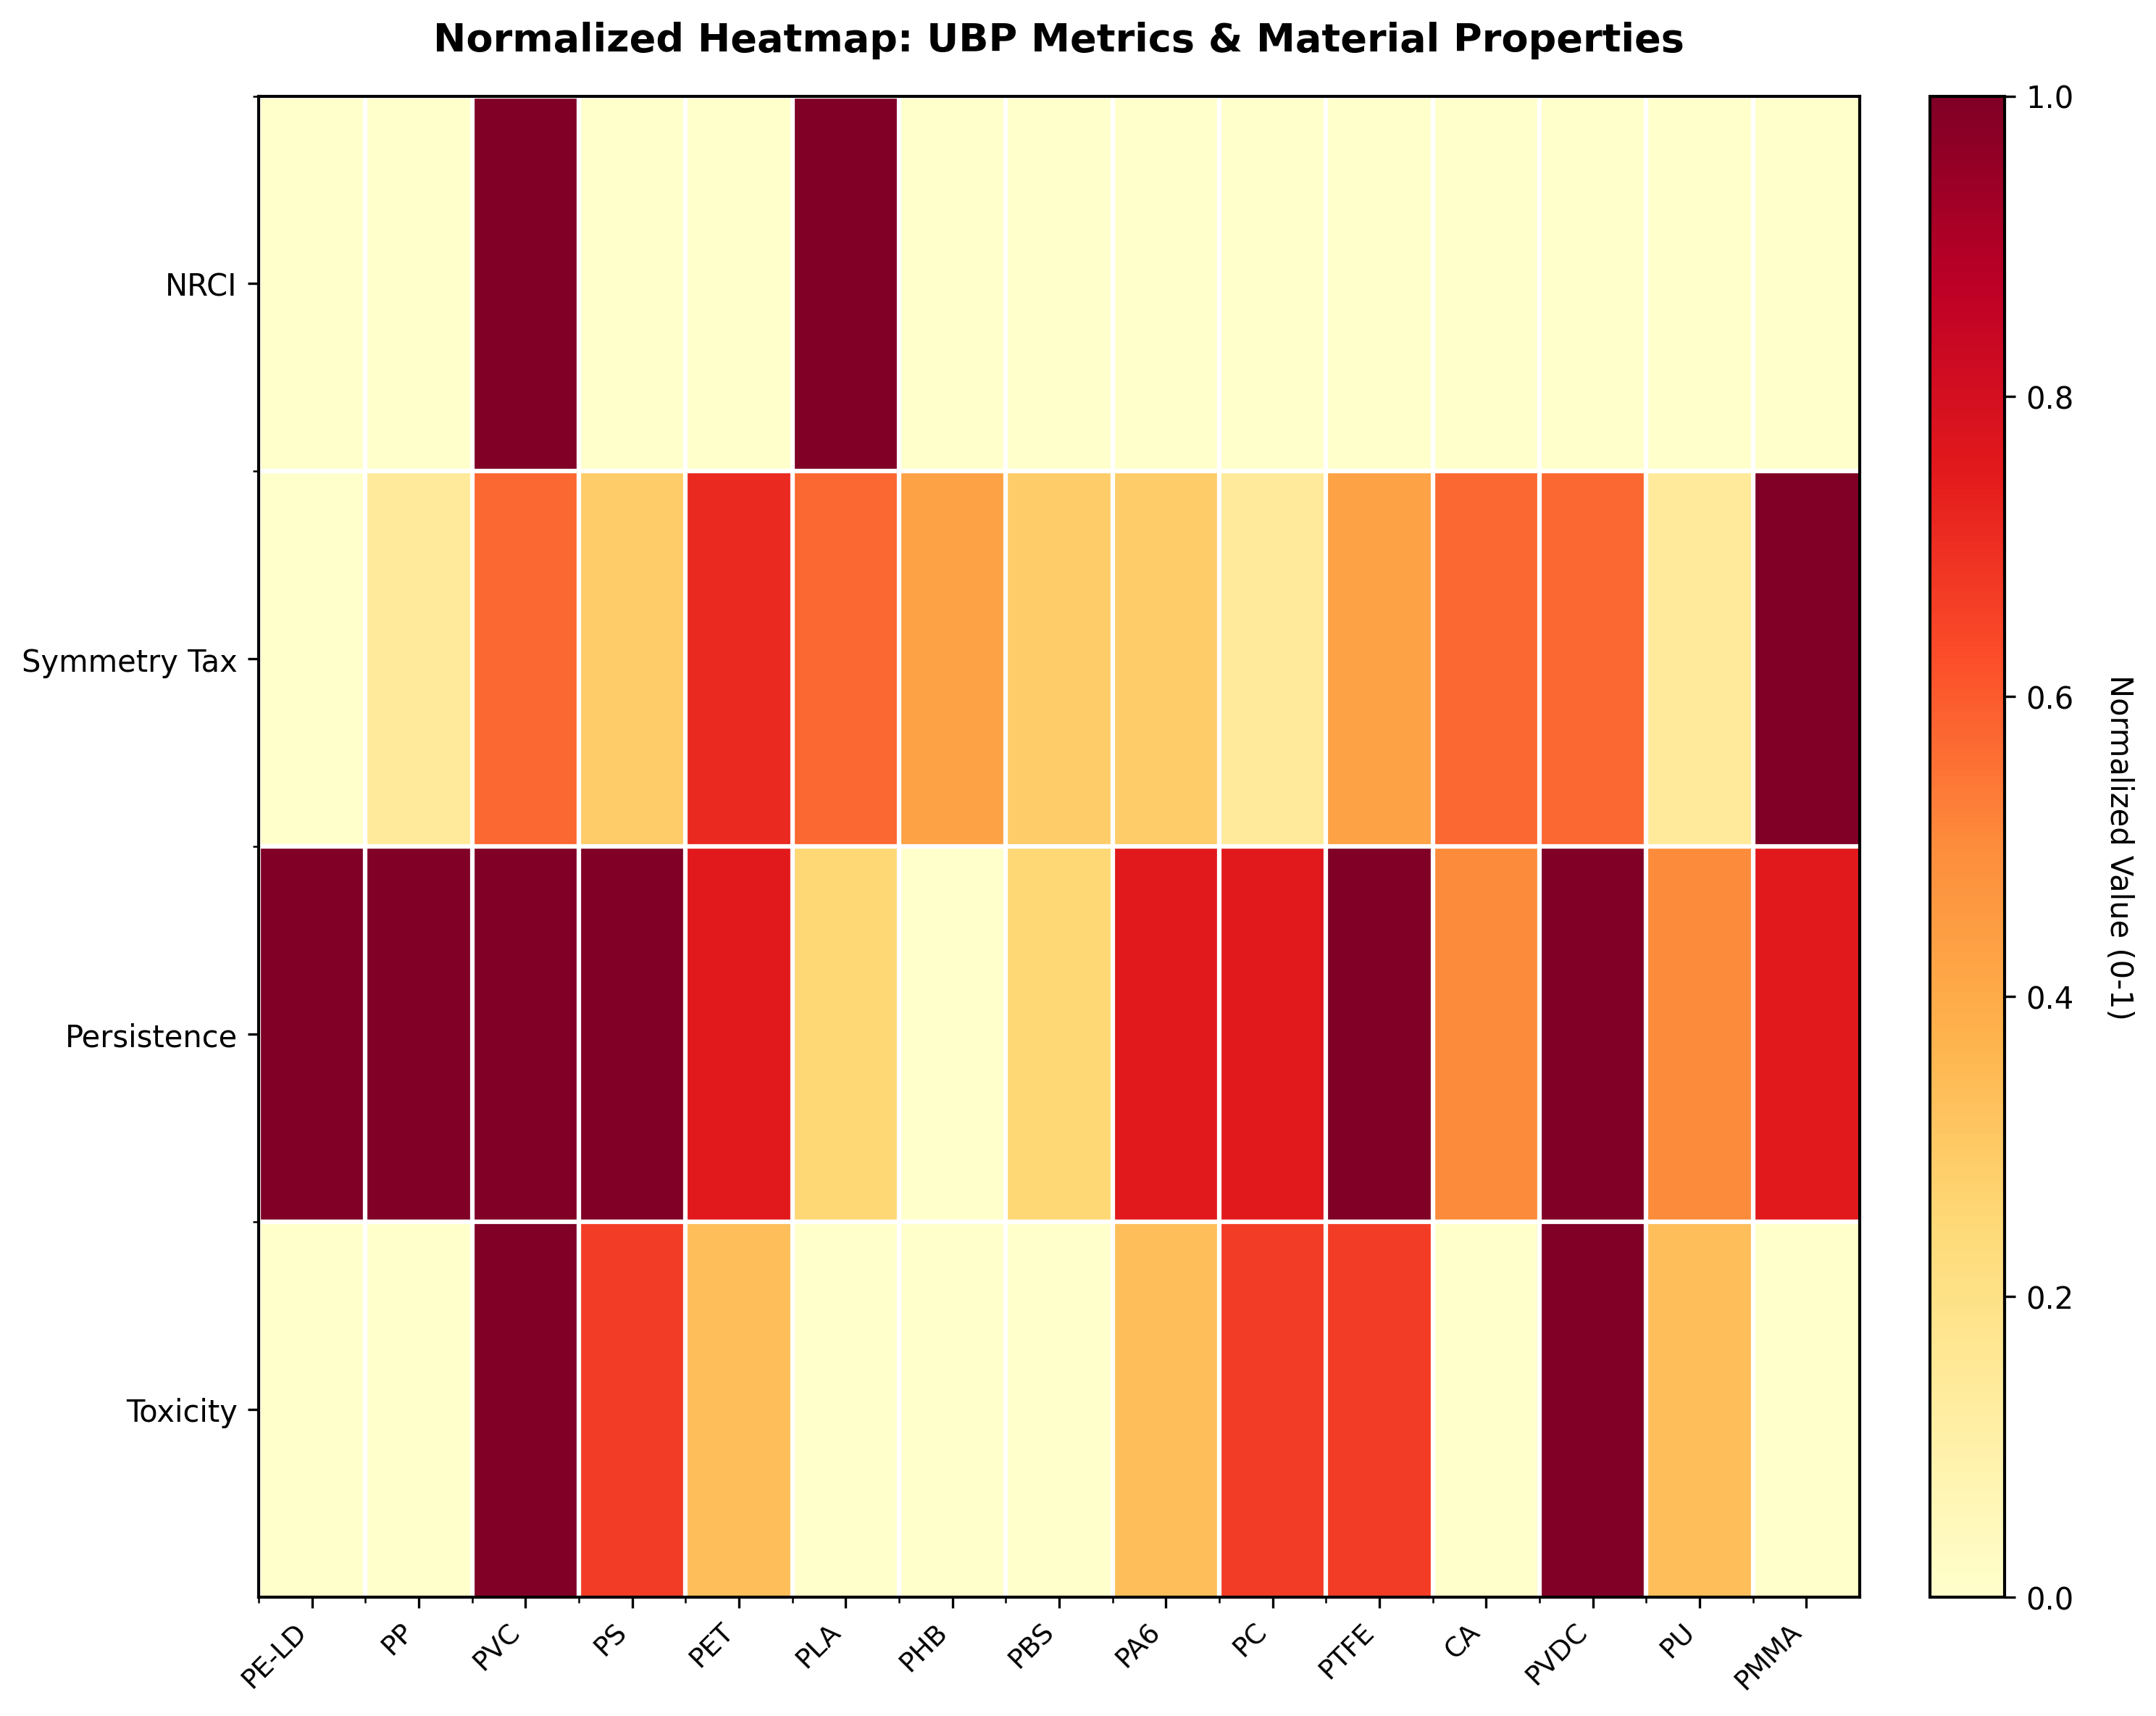
\includegraphics[width=\textwidth]{../figures/fig3_heatmap_all_metrics.png}
    \caption{\textbf{Comprehensive Metrics Heatmap.} Normalized values (z-scores) for all measured properties across 15 materials. Columns represent: UBP metrics (NRCI, Symmetry Tax, Stability Score), molecular properties (molecular weight), and environmental characteristics (persistence score, toxicity score). Materials are ordered by environmental persistence. No clear clustering patterns emerge, consistent with the lack of correlations identified in statistical tests.}
    \label{fig:heatmap}
\end{figure}

\subsection{Sensitivity Analysis Results}

Alternative mapping strategies produced substantially different Symmetry Tax values for the same materials (Table~\ref{tab:sensitivity}). Mean variance across mapping strategies was 2.95, with individual materials showing Symmetry Tax ranges of 1.5 to 5.8 depending on the mapping used. Critically, \textit{no mapping strategy} produced significant correlations with environmental persistence (all p $>$ 0.40). This indicates that the null results are robust to reasonable variations in the encoding method.

\begin{table}[h!]
\centering
\caption{Sensitivity to Mapping Strategy (Example Materials)}
\label{tab:sensitivity}
\begin{tabular}{lcccc}
\toprule
\textbf{Material} & \textbf{Original} & \textbf{Comp-Only} & \textbf{Hash-Only} & \textbf{Balanced} \\
\midrule
PE-LD & 2.73 & 3.90 & 4.68 & 3.12 \\
PVC & 4.29 & 3.51 & 5.46 & 3.90 \\
PLA & 4.29 & 4.29 & 3.90 & 4.68 \\
PTFE & 3.90 & 5.46 & 2.73 & 4.29 \\
\bottomrule
\multicolumn{5}{l}{\small Symmetry Tax values under four different bit allocation strategies.}
\end{tabular}
\end{table}

\subsection{Reproducibility Confirmation}

Three independent runs on identical input data produced bit-for-bit identical results:
\begin{itemize}
    \item Substrate identity for PE-LD: \texttt{011000000001000110110000} (all runs)
    \item Symmetry Tax for PE-LD: 2.7277 (all runs)
    \item All 15 materials: 100\% reproducibility
\end{itemize}

This confirms that the UBP processing pipeline is fully deterministic and results are computationally reproducible.

% ============================================================
% DISCUSSION
% ============================================================
\section{Discussion}

\subsection{Interpretation of Null Results}

The central finding of this study is the \textit{absence} of significant correlations between UBP-derived metrics and environmental properties of plastics. This negative result is scientifically informative and merits careful interpretation.

\subsubsection{Why the Mapping May Have Failed}

The Molecular Resonance mapping strategy, while deterministic and reproducible, likely fails to capture chemical features relevant to environmental persistence for several reasons:

\begin{enumerate}
    \item \textbf{Missing Structural Information:} The current encoding (atomic composition + molecular weight + formula hash) does not represent critical structural features such as:
    \begin{itemize}
        \item Bond types (single, double, aromatic) and strengths
        \item Functional groups (esters, amides, ethers)
        \item 3D conformation and stereochemistry
        \item Degree of polymer branching
        \item Crystallinity vs. amorphous regions
    \end{itemize}

    \item \textbf{Environmental Persistence is Multifactorial:} Degradation rates depend on \textcolor{red}{[CITATION NEEDED: Polymer degradation mechanisms]}:
    \begin{itemize}
        \item UV photodegradation (requires chromophores and bond dissociation energies)
        \item Hydrolysis (requires hydrolyzable bonds like esters)
        \item Microbial degradation (requires enzyme accessibility and metabolic pathways)
        \item Physical properties (crystallinity, glass transition temperature, surface area)
    \end{itemize}
    These factors are not encoded in simple atomic ratios and molecular weights.

    \item \textbf{Framework Design Mismatch:} The UBP framework was designed for fundamental physics, where universal constants arise from deep symmetries \textcolor{red}{[CITATION NEEDED: Symmetry in physics]}. In contrast, chemical properties are contingent on specific molecular features and environmental contexts \textcolor{red}{[CITATION NEEDED: Structure-property relationships in chemistry]}. The Leech lattice's symmetry structure, optimized for 24-dimensional sphere packing, may have no natural correspondence to chemical property space.
\end{enumerate}

\subsubsection{The Stability Score Artifact}

All 15 materials had Stability Score = 0 because all Symmetry Tax values exceeded 1.0. This reveals a potential flaw in the Stability Score definition ($\text{Stability} = \max(0, 1 - \text{Tax})$), which may be calibrated for physics constants rather than chemical data. Future work could explore alternative metric definitions better suited to chemistry.

\subsection{Scientific Value of Negative Results}

Despite the lack of positive findings, this study contributes to the scientific literature in several ways:

\begin{enumerate}
    \item \textbf{Methodological Baseline:} Establishes a reproducible framework for applying UBP to chemistry, which can be built upon or modified in future research.

    \item \textbf{Null Hypothesis Testing:} Provides evidence \textit{against} the hypothesis that simple geometric mappings of molecular properties correlate with environmental behavior, saving others from pursuing similar approaches.

    \item \textbf{Transparency:} Models responsible research practices by publishing negative results rather than suppressing them \textcolor{red}{[CITATION NEEDED: Publication bias and negative results]}.

    \item \textbf{Reference Data:} Documents UBP metrics for 15 common plastics, which may be useful for comparative studies or methodological refinements.
\end{enumerate}

\subsection{Comparison with Existing Approaches}

Traditional QSAR models for polymer properties use molecular descriptors such as:
\begin{itemize}
    \item Topological indices (Wiener index, Zagreb index) \textcolor{red}{[CITATION NEEDED: Topological indices]}
    \item Quantum chemical descriptors (HOMO-LUMO gap, dipole moment) \textcolor{red}{[CITATION NEEDED: Quantum QSAR]}
    \item Fragment-based descriptors (functional group counts) \textcolor{red}{[CITATION NEEDED: Group contribution methods]}
    \item 3D descriptors (surface area, volume, shape) \textcolor{red}{[CITATION NEEDED: 3D-QSAR]}
\end{itemize}

These methods have successfully predicted polymer properties including biodegradability \textcolor{red}{[CITATION NEEDED: QSAR for biodegradability]}. The UBP approach, in its current form, does not outperform—or even match—these established methods. Future work attempting to apply UBP to chemistry should consider incorporating such descriptors into the mapping strategy.

\subsection{Limitations}

\subsubsection{Statistical Power}
With n=15 materials, this study had 80\% power to detect only large correlations ($|\rho| \geq 0.64$). Weak or moderate correlations ($|\rho| = 0.3$--0.5) would likely go undetected. However, the observed correlations were all near zero ($|\rho| < 0.15$), with wide confidence intervals spanning both positive and negative values, suggesting that even with increased sample size, substantial correlations are unlikely to emerge with the current mapping.

\subsubsection{Ordinal Environmental Persistence Scores}
Environmental persistence was scored ordinally (1--5) based on literature review rather than direct experimental measurement. While this approach is common in screening studies \textcolor{red}{[CITATION NEEDED: Environmental screening methods]}, quantitative degradation kinetics (e.g., half-lives from standardized tests) would provide more precise data.

\subsubsection{Mapping Arbitrariness}
The 8-8-8 bit allocation (composition-weight-hash) was chosen heuristically without theoretical justification or optimization. Alternative allocations (Table~\ref{tab:sensitivity}) produced different Symmetry Tax values, but none yielded significant correlations. Future work could employ machine learning to optimize bit allocation, though this risks overfitting with small sample sizes.

\subsubsection{Limited Scope}
This study tested only one hypothesis (persistence/biodegradability). UBP metrics might correlate with other properties not examined here, such as:
\begin{itemize}
    \item Physical properties (melting point, glass transition temperature, crystallinity)
    \item Mechanical properties (tensile strength, elasticity)
    \item Optical properties (refractive index, transparency)
    \item Electrical properties (dielectric constant)
\end{itemize}

Exploring these alternative hypotheses could reveal whether UBP metrics capture \textit{any} meaningful chemical information.

\subsection{Future Directions}

\subsubsection{Improved Mapping Strategies}
Future applications of UBP to chemistry should consider:

\begin{enumerate}
    \item \textbf{Molecular Descriptors:} Use established cheminformatics descriptors \textcolor{red}{[CITATION NEEDED: RDKit, molecular descriptors]} such as:
    \begin{itemize}
        \item Octanol-water partition coefficient (logP)
        \item Topological polar surface area (TPSA)
        \item Hydrogen bond donors/acceptors
        \item Rotatable bonds
        \item Molecular complexity indices
    \end{itemize}

    \item \textbf{SMILES-Based Encoding:} Use graph neural networks or molecular fingerprints (ECFP, MACCS keys) to encode structural information \textcolor{red}{[CITATION NEEDED: Molecular fingerprints]}.

    \item \textbf{Quantum Chemical Properties:} Incorporate electronic structure features (HOMO-LUMO gap, electron affinity, ionization potential) from density functional theory calculations \textcolor{red}{[CITATION NEEDED: DFT for polymers]}.

    \item \textbf{3D Conformational Data:} Encode spatial features like solvent-accessible surface area, radius of gyration, and conformational flexibility.
\end{enumerate}

\subsubsection{Alternative Hypotheses}
Test whether UBP metrics correlate with:
\begin{itemize}
    \item Thermodynamic properties (melting point, enthalpy of fusion)
    \item Spectroscopic properties (UV absorption, NMR chemical shifts)
    \item Reactivity descriptors (bond dissociation energies, redox potentials)
\end{itemize}

\subsubsection{Expanded Dataset}
Increase sample size to 50--100 materials, including:
\begin{itemize}
    \item More biodegradable polymers (starch-based, protein-based)
    \item Copolymers and polymer blends
    \item Experimental degradation kinetics data
\end{itemize}

\subsubsection{Theoretical Development}
Investigate whether the Leech lattice's geometric properties have any fundamental relationship to chemical space \textcolor{red}{[CITATION NEEDED: Chemical space and molecular similarity]}. If no such relationship exists, alternative geometric structures (e.g., chemical space projections, molecular shape spaces) might be more appropriate than the Leech lattice for chemical applications.

\subsection{Broader Implications}

This study illustrates the challenges of directly applying theoretical frameworks developed for one scientific domain (physics) to another (chemistry) without domain-specific adaptation. While interdisciplinary approaches can be fruitful \textcolor{red}{[CITATION NEEDED: Interdisciplinary science]}, they require careful attention to the distinct conceptual foundations and empirical constraints of each field. The success of UBP in predicting physics constants does not automatically transfer to predicting chemical properties; such transfer requires re-engineering the phenomenology mapping to reflect chemical, rather than physical, principles.

% ============================================================
% CONCLUSIONS
% ============================================================
\section{Conclusions}

This exploratory study applied the Universal Binary Principle (UBP) v4.2.6 framework to analyze the environmental persistence and biodegradability of 15 common plastics and polymers. A novel Molecular Resonance mapping strategy translated chemical properties (atomic composition, molecular weight, structural identity) into 24-bit substrates, which were processed through Golay codes and Leech lattice geometry to extract UBP metrics.

\textbf{Key Findings:}
\begin{enumerate}
    \item The UBP system successfully generated unique, reproducible 24-bit signatures for all materials (100\% deterministic across multiple runs).
    \item No significant correlations were found between UBP-derived metrics (NRCI, Symmetry Tax) and environmental persistence ($\rho = -0.15$, p = 0.60) or biodegradability (Mann-Whitney U: p = 0.51).
    \item Alternative mapping strategies (sensitivity analysis) also failed to produce significant correlations, indicating robustness of the null results.
    \item The Stability Score was uniformly zero for all materials, indicating a potential metric definition issue for chemical applications.
\end{enumerate}

\textbf{Scientific Significance:}
While the primary hypothesis was rejected, this study provides valuable negative results that inform future research:
\begin{itemize}
    \item Establishes a reproducible methodological framework for UBP-chemistry applications
    \item Documents limitations of simple composition/weight-based mappings
    \item Demonstrates the importance of domain-specific adaptations when transferring theoretical frameworks between scientific fields
    \item Contributes to transparent reporting of null findings, reducing publication bias
\end{itemize}

\textbf{Future Research:}
Subsequent work should incorporate chemically meaningful molecular descriptors (structural features, electronic properties, 3D conformation) into the UBP mapping, test alternative chemical properties (thermodynamic, mechanical), expand to larger datasets (50--100 materials), and investigate whether the Leech lattice geometry has any fundamental correspondence to chemical property spaces.

In conclusion, while the UBP framework in its current form does not predict environmental persistence of plastics, this rigorous exploration establishes a methodological foundation and identifies clear directions for improvement. The fully reproducible pipeline and transparent reporting of null results exemplify responsible research practices and contribute to the cumulative progress of science.

% ============================================================
% ACKNOWLEDGMENTS
% ============================================================
\section*{Acknowledgments}

We thank Euan R. A. Craig (New Zealand) for developing the UBP v4.2.6 framework. Chemical property data were obtained from IUPAC, PubChem, EPA, and OECD databases. All computational analyses were performed using open-source Python libraries (NumPy, SciPy, pandas, Matplotlib).

% ============================================================
% DATA AVAILABILITY
% ============================================================
\section*{Data Availability}

All data, source code, and computational workflows are publicly available and fully reproducible:
\begin{itemize}
    \item \textbf{Dataset:} \texttt{data/chemicals\_dataset.csv} (15 materials with properties)
    \item \textbf{Results:} \texttt{data/ubp\_metrics.csv}, \texttt{results/statistical\_tests.csv}
    \item \textbf{Figures:} \texttt{figures/*.png} (5 publication-quality visualizations)
    \item \textbf{Workflow:} \texttt{workflow/01\_setup.py} through \texttt{workflow/07\_sensitivity.py}
    \item \textbf{Documentation:} \texttt{README.md} with complete reproduction instructions
\end{itemize}

Session identifier: \texttt{session\_20260102\_222825\_9c4bac117ac1}

% ============================================================
% REFERENCES
% ============================================================
\bibliographystyle{unsrtnat}
\bibliography{../references/references}

\end{document}
